\documentclass[12pt,english]{article}
\usepackage[english]{babel}
\usepackage{graphicx}
\usepackage{amsmath}
\usepackage{multirow}
\usepackage{pgfplots}
\usepackage{subcaption}
\usepackage{amssymb}
\usepackage[hidelinks]{hyperref}
\usepackage{caption}
\usepackage{amsthm}
\usepackage{multicol}
\pgfplotsset{compat=1.16}
\usepackage{minted}
\usepackage{float}
\usepackage{titling}
\usepackage{soul}
\usepackage{listings}
\newenvironment{statement}{\fontfamily{ptm}\selectfont}{\par}
\usepackage{array}
\graphicspath{ {../img/} {./img}}
\selectlanguage{english}
\usepackage[nottoc]{tocbibind}
\usepackage[utf8]{inputenc}
\usepackage{graphicx}
\usepackage[a4paper,left=2cm,right=2cm,top=2.5cm,bottom=2.5cm]{geometry}
\RecustomVerbatimEnvironment{Verbatim}{BVerbatim}{}


\title{Evolutionary Algorithms}
\setlength{\droptitle}{10em}
\author{Carlos Sánchez Páez}

\makeindex
\begin{document}


\begin{titlepage}

\newlength{\centeroffset}
\setlength{\centeroffset}{-0.5\oddsidemargin}
\addtolength{\centeroffset}{0.5\evensidemargin}
\thispagestyle{empty}

\noindent\hspace*{\centeroffset}
\begin{minipage}{\textwidth}

\centering

\includegraphics[width=0.75\textwidth]{bme_logo.jpg}\\[1.4cm]

\textsc{ \Large Evolutionary Algorithms\\[4cm]}

\textsc{\Huge Homework}\\[0.75cm]

{\Large\bfseries Eighth task\\}
\end{minipage}

\vspace{8cm}
\noindent\hspace*{\centeroffset}
\begin{minipage}{\textwidth}
\centering

\textbf{Author}\\ {Carlos Sánchez Páez}\\
\texttt{http://www.github.com/csp98}\\[0.5cm]
\textsc{Budapest University of Technology and Economics}\\
\vspace{1cm}
\textsc{Academic year 2018-2019}
\end{minipage}
\end{titlepage}
\thispagestyle{empty}

\newpage


\begin{enumerate}

	\item
		\begin{statement}
		Design a genetic algorithm to solve the n-queens problem (you don’t have to find every layout, just one where not pairs hit eachother). What sort of crossover and mutation operators would you use? What is the best criterion for stopping? What is a suitable fitness function?
		\end{statement}
		For this problem we will use a permutation representation in the following way:\\
		Each permutation index will represent a column and each element, a row. Let's see an example:
		\begin{center}
			[0,2,3,1]
		\end{center}
		This permutations means that the positions of the queens will be:
		\begin{itemize}
			\item (0,0)
			\item (1,2)
			\item (2,3)
			\item (3,1)
		\end{itemize}
		Which gives us the following board:
		\begin{figure}[H]
			\centering
			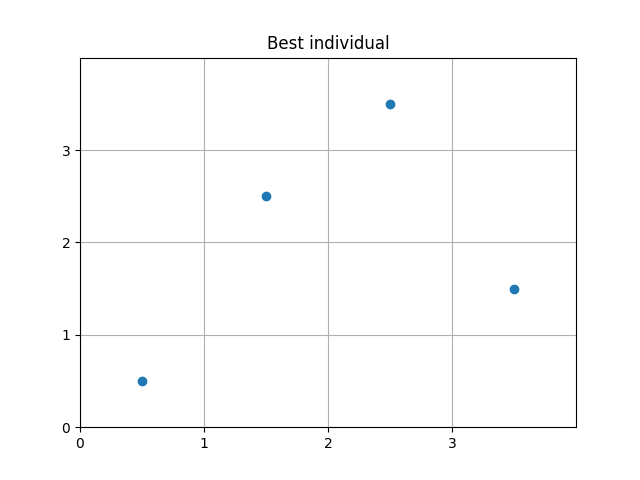
\includegraphics[scale=0.5]{./img/example.png}
		\end{figure}
		As this is an adjacency problem, we need to use the apropiate operators for crossover and mutation. I chose PMX (partially mapped crossover) crossover and inversion mutation.\\

		The fitness functions defines as follows:\\
		The queens won't be on the same row or collumn (they are permutations without repetition, so $p_1(x) \neq p_2(x) \wedge p_1(y) \neq p_2(y)$ $\forall p_i \in P$ with $P$ as the set of all possible permutations).\\
		Thanks to this representation, we don't have to worry about vertical or horizontal attacks between queens: the only possible attacks are the diagonal ones. This means that our fitness function will be the number of queens in a diagonal, if there is more than one.\\
		This makes our problem a minimization one: the permutation with fitness$=0$ is the best one, as there are not attacking queens.\\
		As this problem is a CSP one, we should stop when we find the correct layout (fitness$=0$), which is the feasible one.


	\item
		\begin{statement}
		Find a new example (that is we haven’t mentioned in the class before) for a problem, that can be solve with genetic algorithm using permutation representation. What is the type of it? (CSP-FOP-COP, scheduling-adjacency)? What would be a suitable fitness function?
		\end{statement}
		The \textbf{Minimum Spanning Tree} problem consists on finding a subgraph on a given graph will connects all the vertices, without cycles, with the minimum possible total weight. It is a COP problem, as we have constraints (all the vertices must be reached) and an objective function to minimize (the sum of the weights of the edges).\\
		The permutation representation of the problem should be the following:
		\begin{itemize}
			\item Each elements represents an edge.
			\item 0 means that the edge is not taken.
			\item 1 means that the edge is taken.
		\end{itemize}
		For example, if we have the following graph:
		\begin{figure}[H]
			\centering
			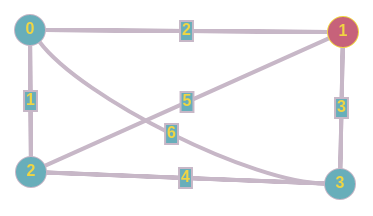
\includegraphics{img/graph}
		\end{figure}
		The permutation
		\begin{center}
			[1,0,1,0,1,0]
		\end{center}
		means that the chosen vertices will be 1,3 and 5, so the spanning tree will be:
		\begin{figure}[H]
			\centering
			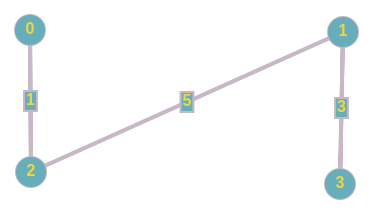
\includegraphics{img/minspan}
		\end{figure}

		Our fitness function should be the sum of the weights of the edges, so we have to minimize it. We also have to check that the individuals are feasible (all the vertices must be reached).


	\item
		\begin{statement}
		Write a program you designed in the first exercise, and examine the running time. What is the maximum size of the chessboard your function can find a good layout? Try different fitness functions (that is different penalties).
		\end{statement}
		My program could find a good layout for 100 queens in 5.28 seconds. It needed 141 generations. However, it could reach bigger sizes.\\
		The running times obtained are represented in the following plot:
		\begin{figure}[H]
			\centering
			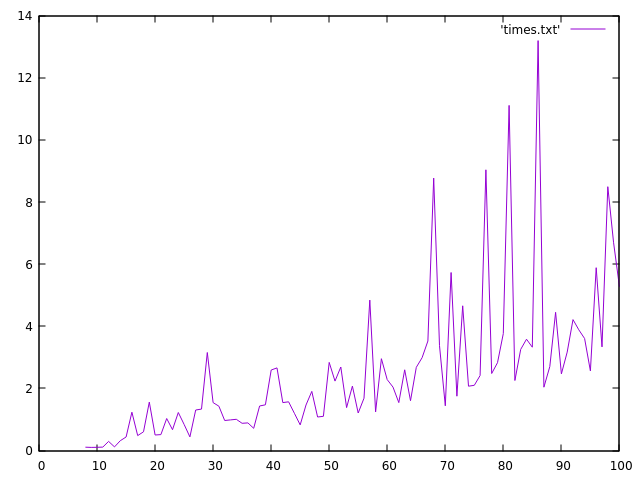
\includegraphics[scale=0.5]{img/plot}
		\end{figure}

		Here is the layout with 100 queens:
		\begin{figure}[H]
			\centering
			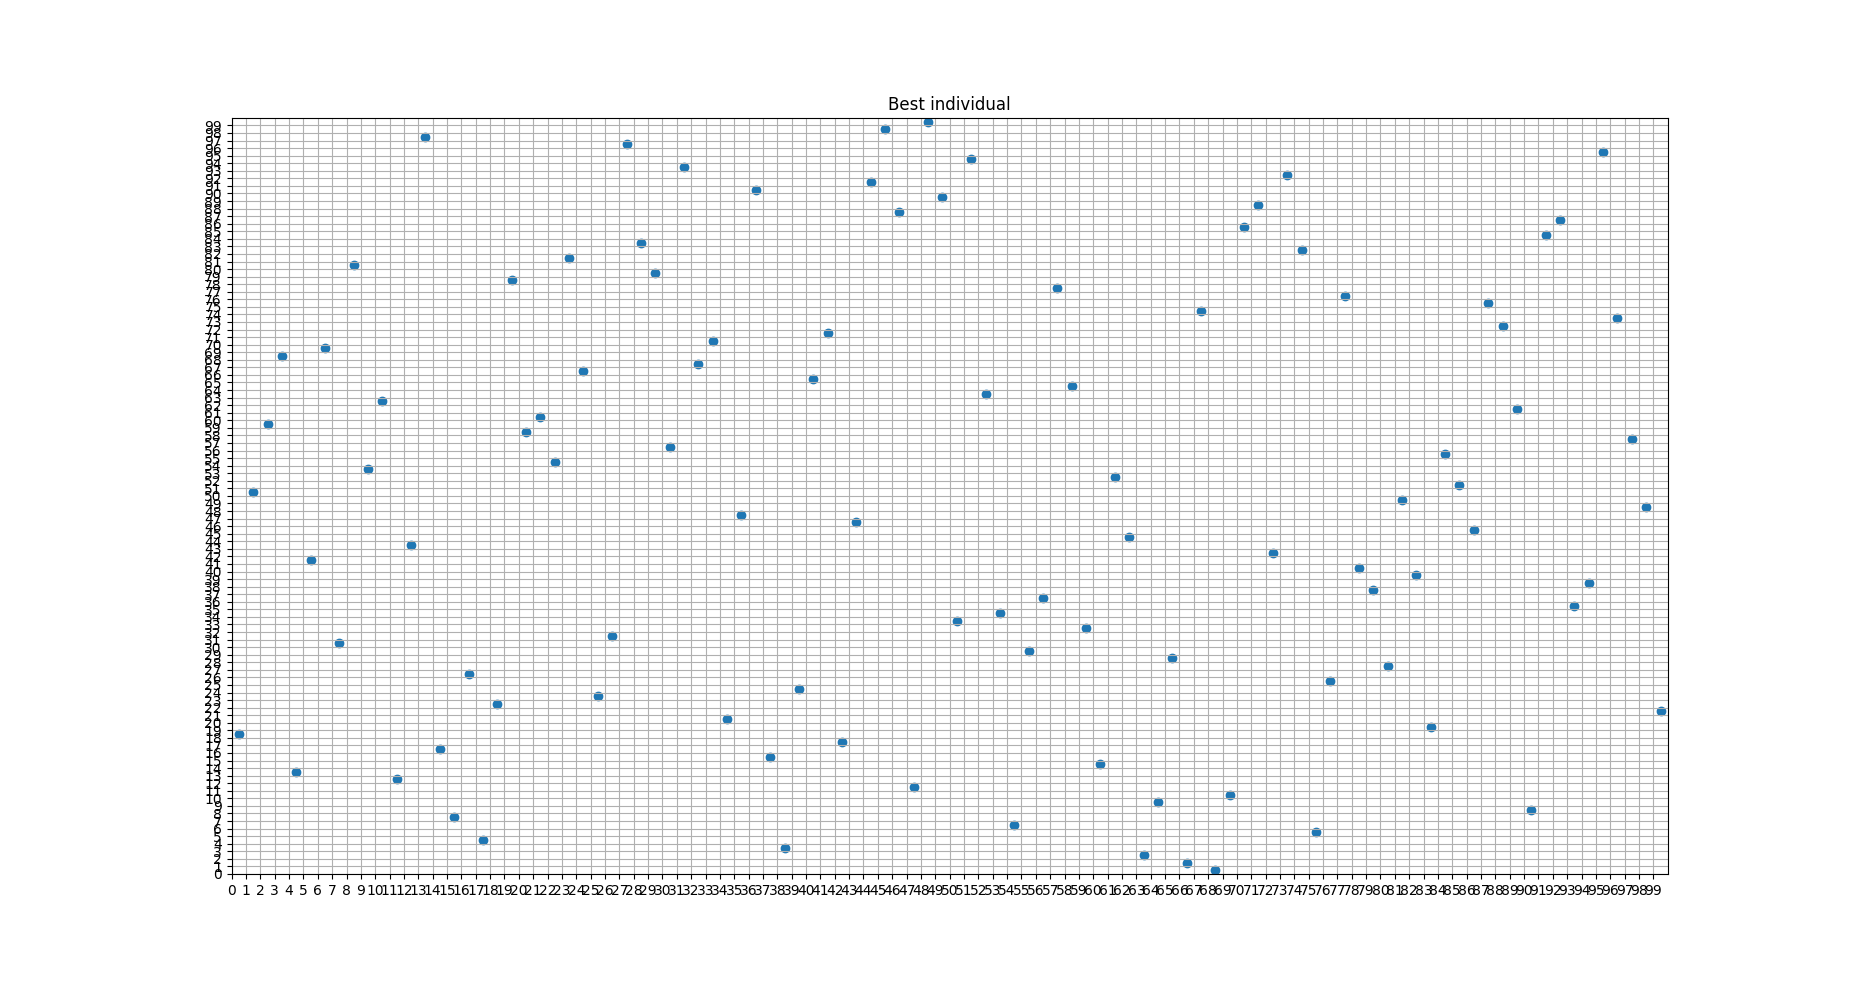
\includegraphics[scale=0.25]{img/100queens}
		\end{figure}


\end{enumerate}


\begin{thebibliography}{9}

\bibitem{Course Webpage}
Course Webpage
\\\texttt{http://math.bme.hu/~safaro/evolalgen.html}


\bibitem{Webpage4}
\texttt{https://tex.stackexchange.com/}


\end{thebibliography}


\end{document}
